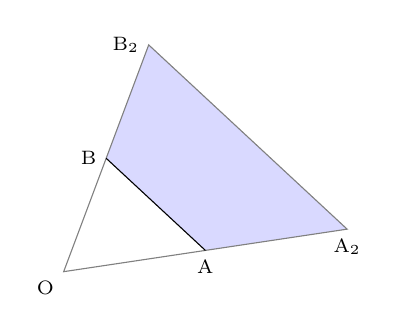
\begin{tikzpicture}[scale=0.9]
\fill[blue!15] (2,0.3)--(4,0.6)--(1.2,3.2)--(0.6,1.6)--cycle;\draw[gray] (0.000,0.000)--(4.000,0.600)--(1.200,3.200)--cycle;\draw[] (2.000,0.300)--(0.600,1.600);\node[below left] at (0.000,0.000){\scriptsize O};\node[below] at (2.000,0.300){\scriptsize A};\node[left] at (0.600,1.600){\scriptsize B};\node[below] at (4.000,0.600){\scriptsize A$_2$};\node[left] at (1.200,3.200){\scriptsize B$_2$};
\end{tikzpicture}